%%
%% ACM SIGCONF survey skeleton (two-column) matching your section plan
%%
\documentclass[sigconf,nonacm]{acmart}

\AtBeginDocument{%
  \providecommand\BibTeX{{Bib\TeX}}%
  \raggedbottom
}

% --- floats (two-column) ---
\setcounter{topnumber}{2}
\setcounter{dbltopnumber}{2}
\renewcommand{\topfraction}{0.9}
\renewcommand{\dbltopfraction}{0.9}
\renewcommand{\textfraction}{0.07}
\renewcommand{\floatpagefraction}{0.85}
\renewcommand{\dblfloatpagefraction}{0.85}

\setlength{\textfloatsep}{8pt plus 2pt minus 2pt}
\setlength{\dbltextfloatsep}{8pt plus 2pt minus 2pt}
\setlength{\floatsep}{6pt plus 2pt minus 2pt}
\setlength{\dblfloatsep}{6pt plus 2pt minus 2pt}
\setlength{\intextsep}{6pt plus 2pt minus 2pt}

% Optional: make the draft less "camera-ready-ish"
\setcopyright{none}
\settopmatter{printacmref=false,printccs=false,printfolios=true}
\acmDOI{}
\acmConference[]{}{}{}
\acmBooktitle{}
\acmISBN{}
\date{}

\makeatletter
\def\@copyrightpermission{}
\def\@acmowned{}
\makeatother

\usepackage{array}
\usepackage{balance}
\usepackage{booktabs}
\usepackage{capt-of}
\usepackage{dblfloatfix}
\usepackage{float}
\usepackage{forest}
\usepackage{makecell}
\usepackage{multirow}
\usepackage{placeins}
\usepackage{ragged2e}
\usepackage{tabularx}
\usepackage{tikz}
\usepackage{xcolor}
\usetikzlibrary{positioning,calc,arrows.meta}

% Custom X-like column
\newcolumntype{Y}{>{\RaggedRight\arraybackslash}X}

% One table formatting macro used everywhere
\newcommand{\tbl}{%
  \scriptsize
  \setlength{\tabcolsep}{4pt}%
  \renewcommand{\arraystretch}{1.12}%
}

\begin{document}

% ======================
% Title + Authors
% ======================
\title[Survey of Data Discovery to Integration in Data Lakes]%
{From Data Discovery to Analytics-Ready Data: A Survey of Search, Preparation, and Integration in Data Lakes}

\author{Sumaiya Azad}
\affiliation{%
  \institution{University of Utah}
  \country{USA}
}

\renewcommand{\shortauthors}{Author et al.}


% ======================
% Abstract
% ======================

\begin{abstract}
Organizations collect many kinds of data in data lakes---for example, spreadsheet-like tables, JSON or XML files, server logs, and fields extracted from documents. Before anyone can run queries or build dashboards, teams must (i)~find the right data sources, (ii)~clean and organize them, and (iii)~line up columns and records across sources so they can be combined.

We review 49 methods published from 2022 to 2025 and group them by what they produce across three phases: \emph{Discovery \& Search} (ranked lists of relevant tables for keyword, join, and union queries), \emph{Preparation \& Wrangling} (cleaned tables and reusable processing workflows), and \emph{Integration \& Matching} (column-to-column matches, record-level entity matches, and merged tables). For each phase, we describe common tasks, system designs, and how methods are evaluated. We also trace what is shared across phases---for example, vector representations (called \emph{embeddings}) trained once and reused for both search and matching. We close with open challenges, including end-to-end evaluation, keeping results up to date as data changes, reliable use of language models for data tasks, and more.
\end{abstract}

% ======================
% CCS Concepts (single block)
% ======================
\begin{CCSXML}
<ccs2012>
 <concept>
  <concept_id>10002951.10003260</concept_id>
  <concept_desc>Information systems~Information integration</concept_desc>
  <concept_significance>500</concept_significance>
 </concept>
 <concept>
  <concept_id>10002951.10003260.10003300</concept_id>
  <concept_desc>Information systems~Data cleaning</concept_desc>
  <concept_significance>500</concept_significance>
 </concept>
 <concept>
  <concept_id>10002951.10003260.10003309</concept_id>
  <concept_desc>Information systems~Data exchange</concept_desc>
  <concept_significance>300</concept_significance>
 </concept>
 <concept>
  <concept_id>10002951.10003260.10003305</concept_id>
  <concept_desc>Information systems~Data mining</concept_desc>
  <concept_significance>300</concept_significance>
 </concept>
 <concept>
  <concept_id>10002951.10003260.10003310</concept_id>
  <concept_desc>Information systems~Data retrieval</concept_desc>
  <concept_significance>300</concept_significance>
 </concept>
</ccs2012>
\end{CCSXML}

\ccsdesc[500]{Information systems~Information integration}
\ccsdesc[500]{Information systems~Data cleaning}
\ccsdesc[300]{Information systems~Data exchange}
\ccsdesc[300]{Information systems~Data mining}
\ccsdesc[300]{Information systems~Data retrieval}


\keywords{data lakes, dataset discovery, table search, join discovery, union discovery, data preparation, data wrangling, data cleaning, schema matching, entity resolution, data integration, analytics-ready data}


\maketitle

% ==========================================================
\section{Introduction}
Data lakes store many kinds of data together---spreadsheet-like tables, semi-structured files (such as JSON or XML), server logs, and fields pulled from documents---without requiring one fixed column layout (called a \emph{schema}) at load time.
Loading data is easy, but using it later is hard.
Before analysts can run queries, build dashboards, or train models, they must (1)~find the right data, (2)~clean and organize it, and (3)~combine it from multiple sources.

\paragraph{Scope and terminology.}
In this survey, \emph{discovery} means finding relevant tables or columns inside a data lake. This includes keyword search and finding tables that can be \emph{joined} (linked by a shared key column, for example matching on \texttt{customer\_id}) or \emph{unioned} (stacked on top of each other because they have similar columns) \cite{10.1145/3555041.3589409,10.14778/3750601.3750694}. \emph{Preparation and wrangling} means cleaning errors, transforming values (for example, converting dates to a standard format), and organizing raw data into usable tables or automated workflows that can run again when new data arrives. \emph{Integration and matching} means lining up columns across different sources (for example, recognizing that \texttt{zip\_code} in one table is the same as \texttt{postal\_code} in another) and producing a single combined output. A special case is \emph{entity resolution (ER)}: deciding whether two records describe the same real-world thing---for instance, whether ``J.\ Smith, NYC'' and ``John Smith, New York'' refer to the same person. We use \emph{analytics-ready data} to mean data that is clean and structured enough to use directly for reports, statistics, or machine learning.

Two trends now make this pipeline harder.
First, modern data lakes are large and weakly documented---tables often lack descriptions, column names are inconsistent, and it is unclear which sources overlap or can be combined \cite{10.1145/3555041.3589409,10.14778/3750601.3750694}.
Second, methods that use \emph{embeddings} (compact numerical vectors that capture the meaning of a column or table) and large language models now appear in all three stages \cite{10.14778/3659437.3659461,10.14778/3611540.3611624,10.14778/3742728.3742757}. These methods can infer what columns mean, suggest cleaning steps, and help match records. But they also raise concerns about cost, reliability, and data privacy.

This survey follows the full path from lake data to analytics-ready outputs in three phases:
(1) \emph{Discovery \& Search} retrieves relevant and joinable or unionable candidates;
(2) \emph{Preparation \& Wrangling} cleans, structures, and transforms selected data into usable tables or rerunnable pipelines; and
(3) \emph{Integration \& Matching} aligns schemas and records to produce unified datasets.
Our methodology uses a six-step process from search to final inclusion.

Our focus is the connection among phases. Instead of treating discovery, preparation, and integration as isolated tasks, we study them as one pipeline where each stage feeds the next.

\paragraph{Contributions.}
\begin{itemize}
  \item We review 49 methods published from 2022 to 2025 in three top database venues (SIGMOD, PVLDB, and ICDE) using a clear process for selecting and categorizing methods (Section~\ref{sec:methodology}).
  \item We propose a taxonomy that groups methods by what they produce---ranked candidate lists, cleaned tables, automated workflows, column matches, or merged datasets---spanning discovery, preparation, and integration (Section~\ref{sec:taxonomy-classes}).
  \item We summarize the tasks, system designs, and evaluation practices in each phase, including trade-offs between effectiveness, cost, and the need for human oversight (Section~\ref{sec:pubs-by-phase}).
  \item We identify open problems, including pipeline-level evaluation, keeping results up to date as data changes, reliable use of language models, fairness and privacy constraints, and the need for shared test collections (Section~\ref{sec:discussion-challenges}).
\end{itemize}


% ==========================================================
\section{Related Work}
\label{sec:related}
Earlier surveys cover \emph{discovery} in data lakes in depth, including keyword search, join discovery (finding tables that share a key column), union discovery (finding tables with compatible columns), indexing (building lookup structures for fast search), and benchmarking (standardized tests for comparing methods) \cite{10.1145/3555041.3589409,10.14778/3750601.3750694}. These surveys clearly define the main discovery tasks and compare systems in detail.

Other work studies individual tasks such as \emph{data cleaning} (fixing errors and inconsistencies), \emph{schema matching} (deciding which columns in two tables refer to the same concept), and \emph{entity resolution} (deciding whether two records describe the same real-world thing) \cite{10.14778/3675034.3675051,10.14778/3742728.3742757,10.1145/3588722}. However, most of these methods focus on one stage at a time and assume data is already somewhat organized. They usually do not show how one stage's output feeds into the next stage in a lake pipeline.

Our survey differs in three ways. First, we assign each method to exactly one phase based on its main output (Section~\ref{sec:methodology}), which avoids double-counting and makes comparisons clearer. Second, we connect discovery, preparation, and integration in one view, showing how each stage depends on the others. Third, we focus on 2022--2025, which lets us capture recent language-model-based methods, newer system designs, and emerging concerns such as cost, reliability, fairness, and privacy.


% ==========================================================
\section{Methodology}
\label{sec:methodology}
This section explains how we found, selected, and organized the methods in this survey. Our goal is a transparent, repeatable process so readers can see exactly which methods are included and why.

\paragraph{Step 1: Research questions.}
For each method we ask four questions: (i)~which phase does it target (discovery, preparation, or integration)? (ii)~what does it mainly produce (for example, a ranked list, a cleaned table, or a merged dataset)? (iii)~what technique does it use? and (iv)~how is it evaluated (which datasets, which metrics, and whether cost is reported)?

\paragraph{Step 2: Search terms.}
We query with \texttt{"data lake" AND (S1 OR S2 OR S3 OR S4)}, where S1--S4 are groups of task keywords (Table~\ref{tab:search-strings}).


% ---------- Table: Search terms ----------
\begin{table}[!htbp]
\caption{Search term groups used for queries over data lakes.}
\label{tab:search-strings}
\centering
\tbl
\begin{tabularx}{\columnwidth}{@{}p{8mm}X@{}}
\toprule
\textbf{ID} & \textbf{Query family (examples of task keywords)} \\
\midrule
S1 & \texttt{discovery}, \texttt{search}, \texttt{table search}, \texttt{dataset retrieval}, \texttt{exploration} \\
S2 & \texttt{joinable}, \texttt{unionable}, \texttt{overlap}, \texttt{join discovery}, \texttt{union discovery} \\
S3 & \texttt{wrangling}, \texttt{preparation}, \texttt{cleaning}, \texttt{transform}, \texttt{pipeline synthesis} \\
S4 & \texttt{schema matching}, \texttt{entity resolution}, \texttt{record linkage}, \texttt{data integration}, \texttt{LLM} \\
\bottomrule
\end{tabularx}
\end{table}

\paragraph{Step 3: Sources and retrieval.}
We scan proceedings of three top database venues---SIGMOD, PVLDB (the journal of the VLDB Endowment), and ICDE---by running title and abstract queries with the keyword groups S1--S4.
The final collection includes 49 methods: 15 from SIGMOD, 22 from VLDB/PVLDB, and 12 from ICDE.

\paragraph{Step 4: Inclusion and exclusion.}
We include methods that study a data lake or lakehouse setting and that propose a concrete technique for discovery, preparation, or integration. We exclude methods that do not target a lake setting.

\paragraph{Step 5: Coding rule.}
Each method is assigned to exactly one phase based on its \emph{primary output}---the main thing it produces. Specifically: a method that outputs a ranked list of candidate tables goes into Discovery; a method that outputs a cleaned table, transformed data, or a reusable processing workflow goes into Preparation; and a method that outputs column matches, record-level entity matches, or a merged dataset goes into Integration. This rule prevents double-counting and makes the taxonomy clear.

\paragraph{Step 6: Synthesis.}
We group all 49 methods by the taxonomy defined in Section~\ref{sec:taxonomy-classes} and summarize the distribution across phases in Table~\ref{tab:taxonomy-summary}. The later literature-review sections describe techniques and evaluation practices within each category.

% ---------- Table: Top-level distribution ----------
\begin{table}[!htbp]
  \caption{Top-level taxonomy distribution.}
  \label{tab:taxonomy-summary}
  \centering
  \tbl
  \begin{tabular}{lr}
    \toprule
    Category & \# Methods \\
    \midrule
    Discovery and Search & 19 \\
    Preparation and Wrangling & 13 \\
    Integration and Matching & 17 \\
    \midrule
    Total & 49 \\
    \bottomrule
  \end{tabular}
\end{table}


\section{Taxonomy Overview}

We organize the 49 methods into a two-level taxonomy. The top level has three \emph{classes}, one for each phase of the pipeline (Discovery, Preparation, Integration). Within each class, we define \emph{categories} that capture common method patterns---for example, ``cleaning and repair'' is one category inside the Preparation class.


% ----------------------------------------------------------
\subsection{Classification Summary}

% ---------- Compact taxonomy diagram ----------
\begin{figure*}[t]
\centering
\scriptsize
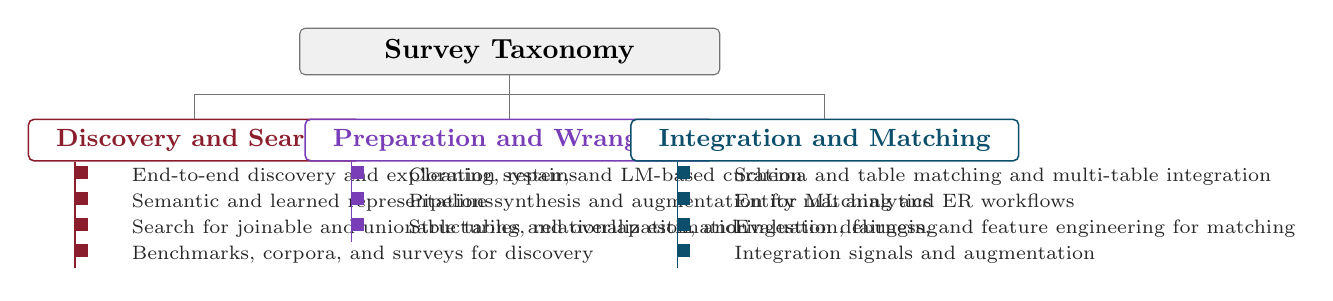
\begin{tikzpicture}[
  font=\scriptsize,
  >=Latex,
  conn/.style={draw=black!55, line width=0.45pt},
  title/.style={draw=black!55, rounded corners=2pt, fill=black!6,
                inner xsep=10pt, inner ysep=4pt, align=center,
                minimum width=0.44\textwidth},
  cat/.style={rounded corners=2pt, fill=white,
              inner xsep=10pt, inner ysep=3.5pt, align=center,
              minimum width=0.26\textwidth, line width=0.55pt},
  itemtext/.style={anchor=west, text=black!85}
]

% Colors
\definecolor{discC}{HTML}{8B1E2D}
\definecolor{prepC}{HTML}{7A3DB8}
\definecolor{inteC}{HTML}{0B4F6C}

% Bullet square size
\def\bs{1.6mm}

\def\gapTop{5.5mm}
\def\barDrop{2.4mm}
\def\stem{2.2mm}
\def\ygap{3.3mm}
\def\xoff{6.0mm}
\def\spineInset{6mm}

% --- Top title ---
\node[title] (root) {\textbf{\normalsize Survey Taxonomy}};

% --- Phase boxes ---
\node[cat, draw=discC, text=discC, below=\gapTop of root, xshift=-0.33\textwidth] (disc)
  {\textbf{\small Discovery and Search}};
\node[cat, draw=prepC, text=prepC, below=\gapTop of root] (prep)
  {\textbf{\small Preparation and Wrangling}};
\node[cat, draw=inteC, text=inteC, below=\gapTop of root, xshift= 0.33\textwidth] (inte)
  {\textbf{\small Integration and Matching}};

% --- Connector bar ---
\coordinate (barC) at ($(root.south)+(0,-\barDrop)$);
\coordinate (barL) at ($(disc.north |- barC)$);
\coordinate (barR) at ($(inte.north |- barC)$);

\draw[conn] (root.south) -- (barC);
\draw[conn] (barL) -- (barR);
\draw[conn] (barL) -- (disc.north);
\draw[conn] (barC) -- (prep.north);
\draw[conn] (barR) -- (inte.north);

% ---------- Discovery ----------
\coordinate (discStem) at ($(disc.south west)+(\spineInset,0)$);
\coordinate (discB1)   at ($(discStem)+(0,-\stem)$);
\coordinate (discB2)   at ($(discB1)+(0,-\ygap)$);
\coordinate (discB3)   at ($(discB2)+(0,-\ygap)$);
\coordinate (discB4)   at ($(discB3)+(0,-\ygap)$);

\draw[conn, draw=discC] (discStem) -- ($(discB4)+(0,-1.4mm)$);

\foreach \p/\txt in {
  discB1/{End-to-end discovery and exploration systems},
  discB2/{Semantic and learned representations},
  discB3/{Search for joinable and unionable tables and overlap estimation},
  discB4/{Benchmarks, corpora, and surveys for discovery}
}{
  \fill[discC] (\p) rectangle ++(\bs,\bs);
  \node[itemtext] at ($(\p)+(\xoff,0.3mm)$) {\txt};
}

% ---------- Preparation ----------
\coordinate (prepStem) at ($(prep.south west)+(\spineInset,0)$);
\coordinate (prepB1)   at ($(prepStem)+(0,-\stem)$);
\coordinate (prepB2)   at ($(prepB1)+(0,-\ygap)$);
\coordinate (prepB3)   at ($(prepB2)+(0,-\ygap)$);

\draw[conn, draw=prepC] (prepStem) -- ($(prepB3)+(0,-1.4mm)$);

\foreach \p/\txt in {
  prepB1/{Cleaning, repair, and LM-based curation},
  prepB2/{Pipeline synthesis and augmentation for ML analytics},
  prepB3/{Structuring, relationalization, and ingestion debugging}
}{
  \fill[prepC] (\p) rectangle ++(\bs,\bs);
  \node[itemtext] at ($(\p)+(\xoff,0.3mm)$) {\txt};
}

% ---------- Integration ----------
\coordinate (inteStem) at ($(inte.south west)+(\spineInset,0)$);
\coordinate (inteB1)   at ($(inteStem)+(0,-\stem)$);
\coordinate (inteB2)   at ($(inteB1)+(0,-\ygap)$);
\coordinate (inteB3)   at ($(inteB2)+(0,-\ygap)$);
\coordinate (inteB4)   at ($(inteB3)+(0,-\ygap)$);

\draw[conn, draw=inteC] (inteStem) -- ($(inteB4)+(0,-1.4mm)$);

\foreach \p/\txt in {
  inteB1/{Schema and table matching and multi-table integration},
  inteB2/{Entity matching and ER workflows},
  inteB3/{Evaluation, fairness, and feature engineering for matching},
  inteB4/{Integration signals and augmentation}
}{
  \fill[inteC] (\p) rectangle ++(\bs,\bs);
  \node[itemtext] at ($(\p)+(\xoff,0.3mm)$) {\txt};
}

\end{tikzpicture}
\caption{Taxonomy of data lake research from discovery and search to analytics-ready outputs via preparation and integration.}
\label{fig:taxonomy}
\end{figure*}


Figure~\ref{fig:taxonomy} shows the three classes and their categories. Together, they reflect the common path from raw lake contents to analytics-ready outputs.

\textbf{Discovery and Search} returns ranked lists of candidate data sources---individual tables, specific columns, or derived views (tables created on-the-fly by joining or filtering existing tables, as in Ver~\cite{10184768})---that help analysts decide what to use next \cite{10184768,10.14778/3681954.3682005}. In this phase, systems must work with incomplete metadata (for example, missing descriptions) and large-lake limits such as index size and search speed. Recent methods combine meaning-based representations, indexes, and search operators to support keyword search and finding joinable or unionable candidates. The actual merge happens later in integration. LakeCompass~\cite{10.14778/3685800.3685880}, CHORUS~\cite{10.14778/3659437.3659461}, and BLEND~\cite{11112882} are representative methods.

\textbf{Preparation and Wrangling} returns cleaned, organized, or transformed datasets (for example, standardized date formats or added columns). It also increasingly returns \emph{runnable workflows} that can be reused when new data arrives. We use this class for three common types of work: cleaning and repair, building pipelines for downstream analytics, and converting messy inputs into structured tables. CtxPipe~\cite{10.1145/3698831} and CM Explorer~\cite{10.14778/3611540.3611595} are representative methods.

\textbf{Integration and Matching} returns alignment results and merged outputs, such as column matches (e.g., \texttt{zip\_code} $\leftrightarrow$ \texttt{postal\_code}), entity matches, and combined tables. This class includes schema matching, entity resolution (ER), and end-to-end workflows that connect discovery, alignment, and integration. FlexER~\cite{10.1145/3588722}, DIALITE~\cite{10.1145/3555041.3589732}, Magneto~\cite{10.14778/3742728.3742757}, and PLM Schema Matching~\cite{10184612} are representative methods.


\subsection{Classes and Their Categories}
\label{sec:taxonomy-classes}
Below, we define each class and its categories. For each class, we state what it produces, then describe the recurring tasks and the kinds of methods we found. The full category breakdown is shown in Figure~\ref{fig:taxonomy}.

In \textbf{Discovery and Search}, methods cluster around four areas: (1)~end-to-end discovery systems that combine indexing and search in one stack, (2)~learned representations (vector embeddings that capture column or table meaning), (3)~search for joinable and unionable candidates (finding tables that can be linked or stacked), and (4)~shared benchmarks and \emph{corpora}---large publicly available table collections, such as GitTables~\cite{10.1145/3588710}, that researchers use to train models and compare results on a common footing.

In \textbf{Preparation and Wrangling}, the categories are: (1)~cleaning and repair (fixing errors and inconsistencies), (2)~pipeline construction for analytics (building automated step-by-step workflows that prepare data for machine learning), and (3)~structuring heterogeneous inputs and debugging ingestion---that is, converting messy files into clean relational tables and diagnosing errors that happen when data is first loaded into the lake.

In \textbf{Integration and Matching}, the categories are: (1)~schema and table matching (lining up columns across tables and merging them), (2)~entity-resolution workflows (deciding which records refer to the same real-world entity), (3)~fairness-aware evaluation (checking whether matching errors are distributed unevenly across demographic groups), and (4)~reusable integration signals (lightweight evidence, such as approximate foreign-key relationships, that can be shared across tasks).

\begin{table*}[!htbp]
\centering
\caption{Survey summary by phase: outputs, recurring tasks, and typical concerns.}
\label{tab:phase-summary}
\tbl
\begin{tabularx}{\textwidth}{@{}p{30mm}p{34mm}Y p{42mm}@{}}
\toprule
\textbf{Phase} & \textbf{Primary output} & \textbf{Recurring tasks} & \textbf{Typical concerns} \\
\midrule
Discovery \& Search &
Ranked candidate tables, columns, views, or augmentations &
Keyword search, joinable and unionable table search, overlap estimation (how much two tables share), interactive exploration, and benchmark construction &
Weak metadata, retrieval quality in large lakes, index maintenance (keeping indexes updated as data changes), and ambiguity during exploration \\
\addlinespace[0.25em]
Preparation \& Wrangling &
Cleaned tables, structured views, changed tables (e.g., standardized dates or added derived columns), or rerunnable workflows &
Repair, transformation recommendation, pipeline synthesis, feature augmentation (adding useful columns), relationalization, and ingestion debugging &
Do-no-harm behavior, repeatability, downstream utility, validation hooks, and changing data conditions \\
\addlinespace[0.25em]
Integration \& Matching &
Column matches (e.g., \texttt{zip\_code} = \texttt{postal\_code}), entity matches or clusters, reusable DI signals, and merged datasets &
Schema matching, entity resolution, filtering and scheduling, augmentation, dependency discovery, and merge rules (\emph{integration semantics}: rules for how partial rows are combined) &
Intent ambiguity, supervision cost, completeness and consistency of outputs, fairness, privacy, and policy constraints \\
\bottomrule
\end{tabularx}
\end{table*}

% ----------------------
\subsubsection{Discovery and Search}
\paragraph{Output.} Ranked candidate data sources (tables, columns, or views) for exploration and enrichment by join or union.

End-to-end systems combine offline enrichment and index maintenance with online retrieval and interaction \cite{10.14778/3685800.3685880,11112882,10.14778/3659437.3659461}.
Representation methods learn column or table embeddings, or sketches, for meaning-based retrieval under weak metadata \cite{10.14778/3587136.3587146,11113165,11113110}.
Join search, union search, and overlap estimation retrieve candidates that can be joined or unioned, then score relatedness for ranking and deduplication \cite{10.14778/3603581.3603587,10.1145/3588689,10.1145/3725365}. These are discovery-time steps: they find candidates but do not produce the final merged table.
Benchmarks and corpora (large shared table collections) support comparable evaluation and training at lake scale \cite{10.1145/3588710,10.14778/3659437.3659448}.


% ----------------------
\subsubsection{Preparation and Wrangling}
\paragraph{Output.} Cleaned or transformed tables, structured relational views, and rerunnable preparation pipelines.

Cleaning and LM-based data curation study repair quality, error reduction, and reusable cleaning workflows \cite{10.14778/3675034.3675051,10.14778/3574245.3574258,10.14778/3611540.3611624,10.14778/3611540.3611628}.
Pipeline synthesis searches operator sequences or added features that improve downstream utility \cite{10.1145/3698831,10.1145/3588945,11113027,10.14778/3603581.3603596}.
Structuring and ingestion debugging turn heterogeneous inputs into tables and diagnose ingestion failures \cite{10.14778/3626292.3626294,10.1145/3665252.3665269,10.14778/3681954.3682019,10.14778/3611540.3611595}.


% ----------------------
\subsubsection{Integration and Matching}
\paragraph{Output.} Column matches (for example, \texttt{zip\_code} $\leftrightarrow$ \texttt{postal\_code}), entity matches/clusters, and merged datasets.

Schema and table integration aligns columns across sets of tables and applies explicit merge rules (\emph{integration semantics}), for example deciding how to fill missing values when different sources provide partial facts \cite{10.1145/3555041.3589732,10.14778/3574245.3574274,10.14778/3742728.3742757,10184612}.
ER workflows combine blocking, matching, and clustering, with attention to supervision cost and intent differences \cite{10.1145/3709715,10.1145/3588722,10.1145/3588712,10.1145/3626711,10.1145/3588938}.
Evaluation work studies filtering speed-versus-quality trade-offs, subgroup fairness results, and low-cost feature signals \cite{10184692,10.14778/3611479.3611525,11112979,10.14778/3681954.3681987}.
Other methods reuse approximate dependency signals, shared embeddings, and selective use of external data \cite{10.1145/3588929,10184556,10.14778/3611479.3611535,10.14778/3603581.3603602}.

These three classes form one pipeline. Discovery reduces a large search space to a manageable candidate set. Preparation converts candidates into stable, reusable outputs. Integration decides how overlaps are aligned and how the final result is produced. This view is useful because many recent methods produce intermediate outputs that flow from one phase to the next.



% ==========================================================
\section{Literature Review}
% ==========================================================

% ----------------------
\subsection{Discovery and Search}
Data discovery and search are the entry point of the lake-to-analytics pipeline. In large repositories with incomplete or unreliable metadata, systems must surface a small set of relevant data sources for exploration or enrichment. In the methods we reviewed, discovery usually combines table understanding, retrieval, and interaction. Table~\ref{tab:discovery-methods} summarizes this phase by category, keywords, and one-line contribution.

\begin{table*}[!htbp]
\caption{Discovery \& Search methods mapped to taxonomy.}
\label{tab:discovery-methods}
\tbl
\begin{tabularx}{\textwidth}{@{}p{24mm}p{28mm}p{18mm}Y@{}}
\toprule
\textbf{Category} & \textbf{Reference} & \textbf{Keywords} & \textbf{Contribution (one line)} \\
\midrule

End-to-end discovery and exploration systems &
CHORUS~\cite{10.14778/3659437.3659461} &
LM, annotation &
Unifies multiple lake discovery/exploration tasks with a foundation-model pipeline and reports consistent gains over task-specific baselines. \\

~ &
BLEND~\cite{11112882} &
plans, ranking &
Defines a declarative discovery-plan abstraction that compiles to improved execution over heterogeneous signals for unified keyword, join, and union discovery with top-$k$ retrieval. \\

~ &
LakeCompass~\cite{10.14778/3685800.3685880} &
indexing, workflows &
End-to-end lake stack for maintenance + search + analysis workflows, with scalable indexing and practical lake operations. \\

~ &
METAM~\cite{10184845} &
utility, ranking &
Ranks candidate datasets by expected downstream task utility (goal-aware profiling + ranking). \\

~ &
Selecting Sub-tables~\cite{10184535} &
sampling, previews &
Selects compact, informative sub-tables to accelerate inspection when full tables are too large or noisy. \\

~ &
Ver~\cite{10184768} &
views, interaction &
Question-driven view discovery that progressively prunes the space to surface useful derived tables. \\

\midrule

Semantic and learned representations &
CMDL~\cite{10.14778/3611479.3611533} &
cross-modal, embeddings &
Learns joint representations to retrieve across structured tables and unstructured text sources for cross-modal dataset discovery. \\

~ &
Starmie~\cite{10.14778/3587136.3587146} &
embeddings, contrastive &
Pretrains contextualized column representations that capture table context to improve semantic dataset discovery, especially unionable-table retrieval. \\

~ &
LIFTus~\cite{11113165} &
fusion, columns &
Learns multi-aspect column representations and adaptively fuses them to boost union search quality across heterogeneous lakes. \\

~ &
TabSketchFM~\cite{11113110} &
sketches, tokens &
Uses compact column sketches with a pretrained tabular model to scale discovery under token/compute constraints. \\

\midrule

Search for joinable and unionable tables and overlap estimation &
DeepJoin~\cite{10.14778/3603581.3603587} &
joinability, retrieval &
PLM-based joinable-table discovery that embeds columns to rank candidate join partners, improving join discovery over lexical baselines. \\

~ &
SANTOS~\cite{10.1145/3588689} &
unionability, semantics &
Relationship-aware semantic union search using relational/context signals to find unionable tables with compatible meaning. \\

~ &
Nested/Joined Lake Search~\cite{10.14778/3681954.3682005} &
nested, joins &
Extends lake search to nested and join-derived candidates not well-modeled as flat standalone tables. \\

~ &
Armadillo~\cite{10.1145/3725365} &
overlap, graphs &
Learns table embeddings whose similarity approximates overlap ratio for fast scalable overlap estimation. \\

\midrule

Benchmarks, corpora, and surveys for discovery &
Rottnest~\cite{11113229} &
indexing, search &
Scalable lake indexing techniques to support efficient search over large, evolving lakes. \\

~ &
GitTables~\cite{10.1145/3588710} &
corpus, benchmark &
Large public corpus of relational tables mined at scale for reproducible training and evaluation. \\

~ &
LakeBench~\cite{10.14778/3659437.3659448} &
benchmark, labels &
Benchmark suite for joinable and unionable table discovery with ground-truth labeling at lake scale. \\

~ &
Data Discovery Survey~\cite{10.14778/3750601.3750694} &
survey, taxonomy &
Consolidates discovery operations (indexes + systems) and evaluation practice, noting gaps in workloads and cost reporting. \\

~ &
Table Discovery Survey~\cite{10.1145/3555041.3589409} &
survey, methods &
Consolidated overview of table discovery methods and open directions at lake scale. \\

\bottomrule
\end{tabularx}
\end{table*}

Overall, discovery methods show four patterns. First, systems are moving from isolated operators to end-to-end discovery stacks. Second, retrieval quality increasingly depends on learned semantic representations instead of metadata alone. Third, search for joinable and unionable candidates and overlap estimation are shared primitives for later integration steps. Fourth, large corpora and benchmarks are central because they make training and comparison more consistent.

Another recurring pattern is that discovery methods treat interaction as part of the core system, not just a UI layer. In large lakes, analysts often start with underspecified needs. Systems therefore support iterative refinement through previews, alternative candidates, and progressive narrowing.

\subsubsection{End-to-end Discovery and Exploration Systems}
End-to-end discovery and exploration systems return \emph{ranked tables, views, or dataset augmentations} (for example, adding useful columns from related tables) that help analysts move from vague intent to an analytics-ready view. A common pipeline has three parts: (i) \emph{offline enrichment} (profiling, meaning labels, vector representations, and keeping indexes up to date), (ii) \emph{online retrieval} (keyword, joinable, unionable, and view search), and (iii) \emph{interactive exploration} for refinement.

\paragraph{Foundation models as a shared backbone for discovery signals.}
CHORUS~\cite{10.14778/3659437.3659461} produces shared semantic signals (e.g., table-class detection, column typing, and join-column prediction) within a foundation-model-driven workflow. These annotations serve as enriched features for indexing/filtering and as guidance for joinability/composability.

Here, foundation models are not only text generators. In CHORUS, one semantic layer supports several discovery tasks. This helps reuse signals, but it also means prompt sensitivity, non-determinism, and cost can affect multiple decisions at once.

\paragraph{Unifying discovery operators with declarative plans.}
BLEND~\cite{11112882} makes this pipeline explicit and tunable with \emph{discovery plans}. These plans are multi-step workflows that mix retrieval, composition, and ranking. They connect offline indexes to online execution and support efficient operator ordering.

\paragraph{Operational stacks that couple maintenance, search, and analysis.}
LakeCompass~\cite{10.14778/3685800.3685880} illustrates this pipeline as an end-to-end lake stack: it maintains tabular data and multiple index structures, supports keyword, join, and union search, and exposes results through APIs and an exploration interface.

\paragraph{Goal-oriented discovery via downstream utility.}
METAM~\cite{10184845} lets downstream task utility steer which candidates and augmentations should be explored next. Rather than ranking only by similarity or joinability, it treats improvements in the target objective as feedback.

\paragraph{Efficient exploration via informative table previews.}
Selecting Sub-tables~\cite{10184535} complements these systems at the interaction layer: even when retrieval returns relevant candidates, tables can be too large to inspect directly. Selecting compact, informative sub-tables under fixed-size/interactive constraints accelerates shortlisting and iteration.

\paragraph{Interaction under ambiguity: view discovery and narrowing.}
Ver~\cite{10184768} studies \emph{view discovery} when many join paths are possible. It searches candidate join structures, removes redundant alternatives, and uses question-driven narrowing to reach the user-intended merged view.

\subsubsection{Semantic and Learned Representations for Discovery}
Discovery is hard in data lakes because \emph{meaning is rarely explicit in metadata}: titles are missing or noisy, schemas are inconsistent, and the same concept appears in many value formats. For this reason, many methods learn vector or sketch representations for columns and tables so retrieval can rely on meaning rather than surface overlap.

\paragraph{Cross-modal embeddings for discovery beyond tables.}
CMDL~\cite{10.14778/3611479.3611533} addresses lakes that combine structured tables with unstructured text by embedding columns and documents into a shared space for cross-modal retrieval. Because explicit cross-modal labels are scarce, it uses weak supervision to generate scalable training signals.

\paragraph{Contextualized column representations for semantic union search.}
Starmie~\cite{10.14778/3587136.3587146} learns \emph{contextualized} column embeddings using self-supervised contrastive pretraining so a column's vector reflects both its values and table context. Retrieval then reduces to nearest-neighbor search in embedding space.

\paragraph{Multi-aspect representations for heterogeneous columns.}
LIFTus~\cite{11113165} targets the fact that many lake columns are not well-modeled as natural language (IDs, patterned strings, measurements). It encodes a column through multiple \emph{aspects} using specialized encoders and adaptively fuses them into a single indexable vector.

\paragraph{Sketch-based neural representations under token and cost constraints.}
TabSketchFM~\cite{11113110} avoids expensive table serialization and token limits by compressing content into sketches that preserve key similarity signals. A transformer is trained to ingest these sketches directly, producing embeddings that support efficient retrieval.

\subsubsection{Join and Union Search, and Overlap Estimation}
Join search, union search, and overlap estimation are tightly connected primitives for \emph{table enrichment}. Starting from a \emph{seed table}, systems retrieve a small set of candidates that can be joined or unioned, then quantify how each candidate relates to the seed. This is still discovery: the system is selecting candidates, not executing final integration.

\paragraph{Joinability and learned retrieval.}
DeepJoin~\cite{10.14778/3603581.3603587} encodes columns into fixed-length vectors with pre-trained language models trained on join signals, then retrieves top-$k$ join partners using ANN indexing. This makes join discovery efficient at lake scale and robust to lexical variation.

\paragraph{Unionability as relational semantic compatibility.}
SANTOS~\cite{10.1145/3588689} models unionability through \emph{inter-column semantic relationships} (from external KBs or a synthesized KB from the lake), helping distinguish true union candidates from tables that merely share surface similarity.

\paragraph{Compositional candidates beyond base tables.}
Nested/Joined Lake Search~\cite{10.14778/3681954.3682005} extends candidate generation by producing and ranking \emph{join-nest} candidates---tables built by combining joins and relationalization steps to match a user's structural intent.

\paragraph{Overlap as the shared scoring primitive.}
Armadillo~\cite{10.1145/3725365} ties these together by providing a unifying measure of relatedness useful \emph{regardless} of whether the integration action is join, union, or deduplication. It formalizes overlap via the \emph{largest overlap} rectangle and normalized \emph{overlap ratio}, then learns graph-based embeddings whose similarity approximates overlap at scale.

\subsubsection{Benchmarks, Corpora, and Surveys for Discovery}
Discovery at lake scale depends on shared resources as much as new ranking models. Corpora support representation learning, benchmarks improve comparability, indexing makes workloads runnable, and surveys clarify tasks and evaluation practice.

\paragraph{Indexing for heterogeneous search workloads.}
Rottnest~\cite{11113229} proposes a lakehouse indexing protocol that manages overheads and consistency, making search-oriented discovery feasible on evolving lake storage.

\paragraph{Corpora for learned discovery.}
GitTables~\cite{10.1145/3588710} curates a large corpus of relational-style tables with semantic-type annotations, supporting representation learning and table-understanding components.

\paragraph{Benchmarks for join and union discovery.}
LakeBench~\cite{10.14778/3659437.3659448} pairs labeled ground truth with workloads that stress both retrieval quality and system efficiency, enabling comparable evaluation across methods.

\paragraph{Operations and indexes perspective.}
The Data Discovery Survey~\cite{10.14778/3750601.3750694} gives an operations-focused view and highlights two common gaps: mismatched evaluation setups and weak cost reporting.

\paragraph{Consolidated overview of table discovery methods.}
The Table Discovery Survey~\cite{10.1145/3555041.3589409} synthesizes discovery techniques and open directions, treating robustness and efficiency as first-class concerns.

Once candidate data sources are surfaced, the next phase focuses on transforming heterogeneous results into usable, cleaned, and structured inputs for analytics and downstream integration.


% ----------------------
\subsection{Preparation and Wrangling}
% ----------------------

Preparation and wrangling convert discovered lake data into analytics-ready representations. Unlike discovery, whose primary output is a ranked candidate set, preparation usually returns (i) a cleaned or repaired dataset, (ii) a transformed or feature-augmented table, or (iii) an executable pipeline that can be rerun as data changes. Table~\ref{tab:prep-methods} groups preparation methods into: (1) cleaning and repair with language-model-based curation, (2) pipeline synthesis and augmentation for ML analytics, and (3) structuring, relationalization, and ingestion debugging.

\begin{table*}[!htbp]
\caption{Preparation \& Wrangling methods mapped to taxonomy.}
\label{tab:prep-methods}
\tbl
\begin{tabularx}{\textwidth}{@{}p{24mm}p{28mm}p{18mm}Y@{}}
\toprule
\textbf{Category} & \textbf{Reference} & \textbf{Keywords} & \textbf{Contribution (one line)} \\
\midrule

Cleaning, repair, and LM-based curation &
Automatic Data Repair~\cite{10.14778/3675034.3675051} &
repair, benchmark &
Benchmarks repair algorithms across datasets/error settings, proposes a repair-search strategy, and distills deployment guidelines. \\

~ &
DataRinse~\cite{10.14778/3611540.3611628} &
transforms, mining &
Recommends semantic data-prep transformations by mining data-preparation code repositories to learn reusable transformation patterns. \\

~ &
Foundation Models for Data Tasks~\cite{10.14778/3574245.3574258} &
LM, prompting &
Casts classical cleaning/integration tasks as prompts and evaluates foundation models, noting strong generalization alongside privacy and domain-specific limitations. \\

~ &
Lingua Manga~\cite{10.14778/3611540.3611624} &
LLM, templates &
Provides a language-model-based curation system with modular templates and orchestration to run end-to-end curation workflows. \\

\midrule

Pipeline synthesis and augmentation for ML analytics &
CtxPipe~\cite{10.1145/3698831} &
pipelines, RL &
Constructs preparation pipelines by conditioning operator selection on dataset/task context and using deep RL to search effective pipelines. \\

~ &
HAIPipe~\cite{10.1145/3588945} &
human-AI, reuse &
Combines human- and machine-generated pipelines via enumeration--sampling (with active learning) and uses RL to search improved AI-pipelines. \\

~ &
Featpilot~\cite{11113027} &
features, joins &
Automatically augments tabular datasets with useful additional features from joinable sources to improve downstream model performance. \\

~ &
Auto-BI~\cite{10.14778/3603581.3603596} &
BI, joins &
Predicts BI schema graphs (joins) via global search, evaluated on large collections of BI models. \\

\midrule

Structuring, relationalization, and ingestion debugging &
Evaporate~\cite{10.14778/3626292.3626294} &
views, synthesis &
Uses language models plus lightweight synthesis and weak supervision to generate structured views over heterogeneous lake inputs. \\

~ &
Auto-Tables~\cite{10.1145/3665252.3665269} &
relationalization, schema &
Relationalizes semi-structured tables without examples by inferring structure/schemas and producing normalized relational output. \\

~ &
ReCG~\cite{10.14778/3681954.3682019} &
JSON, clustering &
Discovers JSON schemas bottom-up by clustering records and generalizing clusters into schema fragments. \\

~ &
CM Explorer~\cite{10.14778/3611540.3611595} &
validation, debugging &
Disentangles correlated violated conditional unit tests using graph-based exploration to localize ingestion errors. \\

~ &
XDBC~\cite{10.1145/3725294} &
transfer, tuning &
Decomposes data transfer into configurable stages and auto-tunes configurations for heterogeneous systems to improve throughput. \\

\bottomrule
\end{tabularx}
\end{table*}

Across these methods, preparation is less about one cleaning operator and more about producing reusable outputs under changing conditions. Some methods focus on reducing errors. Others build workflows that improve downstream models. Others convert heterogeneous inputs into structured tables that can be validated and reused. The common theme is repeatable workflows instead of one-time manual steps.

This phase sits in the middle of the pipeline. Discovery often retrieves promising but messy data, while integration assumes some regularity in structure and values. So preparation methods do more than improve local cleaning quality: they directly affect how well later matching and integration work. This role is easy to miss when evaluation reports only local repair or transformation metrics.



\subsubsection{Cleaning, Repair, and LM-based Curation}
Data lakes exacerbate classic data-quality issues: errors are frequent and heterogeneous, and the context needed to
interpret dirty values is often missing. Work in this category focuses on (i) \emph{deployable} repair that
actually reduces errors (not just edits cells), and (ii) \emph{reusable} curation workflows that capture preparation
know-how as controllable operators.

Preparation methods also optimize different goals. Some target consistency under constraints. Some target net error reduction in the final repaired table. Others are judged by downstream model quality. The automatic data repair survey shows why mixing these goals without saying so can mislead evaluation \cite{10.14778/3675034.3675051}. In data lakes, this matters because the workflow that improves consistency is not always the one that best supports later integration or analytics.

\paragraph{Deployment-aware objectives and evaluation.}
Automatic Data Repair~\cite{10.14778/3675034.3675051} argues for error-reduction-oriented objectives and metrics, and benchmarks repair methods across datasets and error settings, including strategies that mitigate \emph{incorrect repairs} so that repair does not introduce new errors.

\paragraph{Prompting-based wrangling and its constraints.}
Foundation Models for Data Tasks~\cite{10.14778/3574245.3574258} casts classical data tasks (cleaning, integration, transformation) as prompted interactions by linearizing structured data into text. The study shows where foundation models generalize well across tasks, while also surfacing practical constraints---notably privacy exposure and sensitivity to domain-specific conventions.

\paragraph{Reusable LM-based curation workflows.}
Lingua Manga~\cite{10.14778/3611540.3611624} operationalizes language-model-based curation by providing a system layer where users compose pipelines with a small DSL and templates. Its design targets cost and repeatability by reducing expensive model calls and supporting workflows that can be run again when new lake data arrives.

\paragraph{Mining semantic transforms from preparation code.}
DataRinse~\cite{10.14778/3611540.3611628} mines semantic transformation patterns via static analysis of code, groups related field-level expressions so suggestions remain coherent, and frames assistance as human-in-the-loop recommendations.



\subsubsection{Pipeline Synthesis and Augmentation for ML Analytics}
Pipeline synthesis treats data preparation as a \emph{utility-driven search} problem. Given raw tables and a downstream ML or analytics objective, the system constructs an executable sequence of cleaning, transformation, and feature operators under cost constraints.

\paragraph{Context-conditioned pipeline construction.}
CtxPipe~\cite{10.1145/3698831} reduces blind search in a very large pipeline space. It uses dataset context and task feedback to choose operators and prioritize transformations that are more likely to improve model utility.

\paragraph{Hybrid human--machine pipeline generation.}
HAIPipe~\cite{10.1145/3588945} combines human-authored pipelines with machine-generated candidates: it uses the human pipeline as a strong prior and augments it with automatically discovered steps, aiming to improve effectiveness while keeping the resulting pipeline aligned with domain expectations.

\paragraph{Feature augmentation via join-path search.}
Featpilot~\cite{11113027} automatically augments a base training table with external features accessible through joinable tables, including \emph{multi-hop} join paths. It ranks candidate augmentations by jointly considering integration quality/coverage and predictive value.

\paragraph{From pipelines to analytics products.}
Auto-BI~\cite{10.14778/3603581.3603596} targets BI-ready structures by synthesizing the \emph{join model} needed to connect multiple tables for analysis. It predicts joins by using local join evidence and a global schema graph.



\subsubsection{Structuring, Relationalization, and Ingestion Debugging}
This category covers methods that convert heterogeneous lake inputs into analyzable structure and methods that keep that
structure trustworthy under imperfect ingestion and cross-system movement.

\paragraph{LM-enabled structured views over heterogeneous inputs.}
Evaporate~\cite{10.14778/3626292.3626294} aims to build a queryable table from a document collection while controlling cost and coverage. It produces a structured view (attributes plus one row per document) and studies two strategies: direct extraction and code synthesis. It also includes an extended variant that combines synthesized extractors using weak supervision.

\paragraph{Example-free relationalization of tables in the wild.}
Auto-Tables~\cite{10.1145/3665252.3665269} frames relationalization as synthesizing a multi-step transformation program (e.g., slicing, header normalization, reshaping) that converts non-relational inputs into standard relational form without user-provided input--output examples.

\paragraph{Schema induction for semi-structured collections.}
ReCG~\cite{10.14778/3681954.3682019} discovers a usable schema bottom-up: it clusters records with similar structure, generalizes clusters into schema fragments, and merges fragments into a compact global schema using an MDL-style objective.

\paragraph{Ingestion debugging with conditional data unit tests.}
CM Explorer~\cite{10.14778/3611540.3611595} proposes conditional data unit tests that target subsets of the data rather than only global aggregates. To avoid redundant alarms, it supports interactive exploration over an entity--tuple graph to disentangle correlated test failures and pinpoint likely erroneous tuples.

\paragraph{Data movement as a configurable transfer pipeline.}
XDBC~\cite{10.1145/3725294} provides a transfer pipeline with reader and writer interfaces and staged steps (read, deserialize, compress, send and receive, decompress, serialize, write). Its components have multiple physical implementations; a heuristic tuner auto-tunes configurations to reduce manual tuning and improve throughput.


% ----------------------
\subsection{Integration and Matching}

Integration and matching align and merge heterogeneous sources to produce analytics-ready views. The output moves from ``cleaner inputs'' to explicit correspondences (schema matches and entity matches) and a merged dataset. In data lakes, weak metadata, partial overlaps, missing values, and ambiguous intent make this harder. Table~\ref{tab:integration-methods} summarizes integration and matching methods.

\begin{table*}[!htbp]
\caption{Integration \& Matching methods mapped to taxonomy.}
\label{tab:integration-methods}
\tbl
\begin{tabularx}{\textwidth}{@{}p{24mm}p{28mm}p{18mm}Y@{}}
\toprule
\textbf{Category} & \textbf{Reference} & \textbf{Keywords} & \textbf{Contribution (one line)} \\
\midrule

Schema and table matching and multi-table integration &
DIALITE~\cite{10.1145/3555041.3589732} &
open-data, alignment &
End-to-end pipeline that discovers relevant open tables and integrates them by aligning schemas/values (KG+LLM-assisted). \\

~ &
ALITE~\cite{10.14778/3574245.3574274} &
integration, disjunction &
Adaptive-learning approach for integrating discovered lake tables under full-disjunction semantics at scale. \\

~ &
Magneto~\cite{10.14778/3742728.3742757} &
matching, hybrid-LM &
Hybrid schema-matching system: a small LM proposes candidate matches and a large LM verifies/repairs hard cases. \\

~ &
PLM Schema Matching~\cite{10184612} &
matching, embeddings &
Adapts pre-trained LMs to encode attribute/column semantics for schema matching across heterogeneous schemas. \\

\midrule

Entity matching and ER workflows &
FlexER~\cite{10.1145/3588722} &
ER, intents &
Models ER with multiple downstream intents as multi-label classification and uses a multiplex-graph GNN for intent-aware matching. \\

~ &
Progressive EM~\cite{10.1145/3709715} &
progressive, scheduling &
Characterizes the design space of progressive EM and benchmarks progressive strategies including NN/PLM-based variants. \\

~ &
Unicorn~\cite{10.1145/3588938} &
multitask, matching &
Unified multi-task model supporting several DI matching tasks via shared encoders and task-specific heads. \\

~ &
WeakSup GT Inference~\cite{10.1145/3588712} &
weak-supervision, labels &
Infers latent ground truth from weak supervision sources by learning a label model that combines noisy signals for EM. \\

~ &
Battleship~\cite{10.1145/3626711} &
active-learning, low-resource &
Active-learning approach for low-resource EM that selects informative pairs via a Battleship-style strategy. \\

\midrule

Evaluation, fairness, and feature engineering for matching &
Fairness Lens~\cite{10.14778/3611479.3611525} &
fairness, bias &
Audits EM through fairness by constructing social datasets and analyzing disparate error rates under imbalance. \\

~ &
Filtering Benchmarks~\cite{10184692} &
blocking, benchmark &
Benchmarks combinations of filtering and scheduling strategies for (progressive) ER across datasets. \\

~ &
DescSim Rules~\cite{11112979} &
rules, features &
Introduces description-similarity rules to engineer informative, interpretable EM features from attribute descriptions. \\

~ &
Relation Enrichment~\cite{10.14778/3681954.3681987} &
enrichment, attributes &
Boosts ER quality by enriching related tuples with additional attributes from auxiliary sources. \\

\midrule

Integration signals and augmentation &
Causal DI~\cite{10.14778/3603581.3603602} &
causal, confounders &
Defines causal data integration (CDI): augments datasets with missing confounders from external sources and infers a causal graph. \\

~ &
Entity Augmentation~\cite{10.14778/3611479.3611535} &
augmentation, querying &
Studies how to augment entities by selectively querying external sources with cost-aware querying strategies. \\

~ &
Sudowoodo~\cite{10184556} &
contrastive, representations &
Self-supervised contrastive approach that learns similarity-aware representations from unlabeled data and transfers to multiple DI tasks. \\

~ &
SIND~\cite{10.1145/3588929} &
dependencies, profiling &
Discovers similarity inclusion dependencies (approximate containment/foreign-key-like signals) to reveal join/integration opportunities. \\

\bottomrule
\end{tabularx}
\end{table*}

The integration literature splits into a few recurring concerns. One set of methods studies schema-level alignment and merge semantics. A second set studies entity resolution as a workflow with blocking, matching, and clustering choices. A third set studies careful evaluation, including fairness and feature design. A fourth set produces reusable signals and augmentation strategies that support multiple integration tasks.

Across these concerns, there is a broader shift: integration is no longer viewed as only a final merge step. Many recent methods treat integration outputs as reusable evidence for candidate generation, prioritization, verification, and downstream analytics. In this view, integration both consumes outputs from earlier phases and produces signals that feed back into discovery and preparation.


\subsubsection{Schema and Table Matching and Integration}
\label{sec:lit-sm-integration}

Schema-level and table-level matching form the \emph{alignment core} of lake integration. Given a set of discovered tables, systems infer column matches under weak metadata and apply merge rules (\emph{integration semantics}) to build one analysis-ready table. This is different from join and union search: here the system actually performs multi-table integration and produces a final merged output.

\paragraph{End-to-end pipelines.}
DIALITE~\cite{10.1145/3555041.3589732} treats integration as a workflow:
\emph{discover} relevant tables $\rightarrow$ \emph{align \& integrate} them $\rightarrow$ \emph{analyze} the merged table.
Different discovery methods can feed the same alignment/integration stage.
Its intermediate outputs (candidate set, alignments, merged output) support iterative validation.

\paragraph{Integration semantics and operators.}
ALITE~\cite{10.14778/3574245.3574274} argues that integration quality depends on clear merge semantics, not only pairwise joins.
It does \emph{global} matching to assign \emph{integration IDs} (shared IDs mark matched columns), then applies
\emph{Full Disjunction (FD)} to combine partial facts across sources.
ALITE breaks FD into reusable operators---\emph{outer union}, \emph{subsumption}, and \emph{complementation}---for null-heavy, partially overlapping tables.

This focus on semantics is also central in DIALITE~\cite{10.1145/3555041.3589732}. The core idea is to connect partial facts across sources, not just run local joins. Discovery is only the first step; the harder step is aligning and combining tables so the final output is useful for analysis.

\paragraph{LM-powered schema matching.}
Magneto~\cite{10.14778/3742728.3742757} uses a hybrid retrieve-then-verify design: a smaller LM proposes/ranks candidates and a larger LM validates/reranks for higher precision under cost constraints. PLM Schema Matching~\cite{10184612} targets enterprise settings with limited access to records and large, domain-specific target schemata, using PLMs with data-efficient adaptation to reduce labeling effort.


\subsubsection{Entity Matching and ER Workflows}

Entity matching (EM), also called entity resolution (ER), record linkage, or deduplication, identifies records that refer to the same real-world entity and outputs
match links or entity clusters. In data lakes, EM is typically embedded in a workflow because tables are discovered
opportunistically, schemas are inconsistent, and entity descriptions mix structured attributes with free text.

\paragraph{Workflow perspective.}
A standard ER pipeline includes (i) filtering/blocking to shrink the comparison space, (ii) pairwise matching to score/classify candidates, and (iii) clustering to enforce global consistency (e.g., transitivity).

\paragraph{Progressive and intent-aware matching.}
Progressive EM~\cite{10.1145/3709715} studies pay-as-you-go ER with four steps: filtering, weighting, scheduling, and matching. The goal is to run high-yield comparisons early when resources are limited. FlexER~\cite{10.1145/3588722} shows that match criteria can change with downstream intent and models this as multi-label classification.

\paragraph{Lowering supervision cost and unifying models.}
WeakSup GT Inference~\cite{10.1145/3588712} combines noisy weak supervision signals with a label model that enforces global constraints (for example, transitivity). This improves training labels with limited manual work. Battleship~\cite{10.1145/3626711} targets low-resource settings with active learning that selects informative pairs. Unicorn~\cite{10.1145/3588938} uses one shared model with task-specific heads to support multiple matching tasks.


\subsubsection{Evaluation, Fairness, and Feature Engineering for Matching}

Beyond reporting overall F1, recent EM/ER work treats matching as a configurable, accountable pipeline component: filtering determines which pairs are even considered, subgroup behavior can diverge under sensitive attributes, and lightweight feature/attribute augmentation can improve accuracy without full retraining.

\paragraph{Benchmarking filtering under quality--runtime targets.}
Filtering Benchmarks~\cite{10184692} compares blocking workflows against nearest-neighbor retrieval for candidate generation and shows that meaningful comparisons require tuning many interacting parameters. Its evaluation reports effectiveness alongside time efficiency and scalability.

\paragraph{Fairness-aware evaluation for EM.}
Fairness Lens~\cite{10.14778/3611479.3611525} audits EM methods across demographic subgroups and shows how disparities can surface under common data conditions such as group imbalance. By advocating fairness-sensitive metrics beyond population-averaged scores, it makes visible failure modes that global metrics can mask.

\paragraph{Practical feature selection and attribute enrichment.}
DescSim Rules~\cite{11112979} mines interpretable similarity rules that incorporate attribute descriptions and value-distribution statistics, pushing expensive retraining to an offline stage. Relation Enrichment~\cite{10.14778/3681954.3681987} treats missing context as a controllable lever by selecting a small set of diverse, low-null auxiliary attributes to strengthen a downstream ER model.


\subsubsection{Integration Signals and Augmentation}
\label{sec:integration-signals}

Recent data-lake integration work emits \emph{reusable signals} (e.g., relaxed dependencies or learned similarity spaces) and supports \emph{targeted augmentation}
from external sources. These outputs act as lightweight evidence to prioritize candidate joins and enrich sparse tables only when needed.

\paragraph{Relaxed dependency signals for noisy join discovery.}
SIND~\cite{10.1145/3588929} introduces similarity inclusion dependencies (sINDs), which relax classical INDs by requiring sufficiently similar counterparts rather than exact value containment. sINDs provide foreign-key-like \emph{joinability hints} that remain informative under typos and formatting variation.

\paragraph{Reusable representation signals across DI and preparation tasks.}
Sudowoodo~\cite{10184556} pre-trains similarity-aware representations via contrastive self-supervision on unlabeled data and applies them across multiple DI tasks under a matching-based formulation. The learned embedding space supports high-recall candidate generation while optional fine-tuning reduces labeled-data needs.

\paragraph{On-demand external enrichment via progressive querying.}
Entity Augmentation~\cite{10.14778/3611479.3611535} studies enrichment when external sources are accessible only through keyword-search interfaces. It proposes a progressive, feedback-driven strategy for retrieving entity-relevant information efficiently.

\paragraph{Analysis-driven augmentation for causal validity.}
Causal DI~\cite{10.14778/3603581.3603602} frames augmentation around causal requirements: it seeks missing confounders from external sources and constructs a causal graph to identify sufficient adjustment sets for causal queries. This produces enriched attributes and explicit dependency structure that guides what to integrate.


\section{Publications by Phase}
\label{sec:pubs-by-phase}

Table~\ref{tab:taxonomy-summary} shows a balanced distribution across phases: Discovery \& Search has 19 methods (38.8\%), Preparation \& Wrangling has 13 (26.5\%), and Integration \& Matching has 17 (34.7\%). Venue coverage is broad: 22 methods from VLDB/PVLDB, 15 from SIGMOD, and 12 from ICDE. Overall, recent data-lake work is not limited to isolated tasks. Discovery methods increasingly report full system stacks and shared benchmarks. Preparation methods often produce rerunnable workflows or structured outputs. Integration methods increasingly emphasize workflow design, intent, and evaluation beyond one global score. A strong cross-phase pattern is reuse of shared signals such as learned representations, profiling cues, and intermediate matching evidence.

\paragraph{Discovery and Search.}
The discovery subset is slightly larger than the other two phases, which is consistent with the practical difficulty of navigating large lakes before any cleaning or alignment can begin. Within this phase, recent work spans both operational systems and shared resources such as corpora (shared table collections), benchmarks, and embedding methods. That mix matters because retrieval quality in large lakes depends not only on better ranking models, but also on the availability of shared resources for training and comparison.

\paragraph{Preparation and Wrangling.}
The preparation subset is smaller, but it covers a wide range of outputs. Some methods repair values or recommend transformations, some synthesize reusable workflows, and others convert heterogeneous inputs into relational structure. This diversity suggests that preparation is still less standardized than discovery or entity matching. At the same time, it also shows why preparation remains central: downstream integration quality depends heavily on whether the selected data can be normalized, validated, and reused.

\paragraph{Integration and Matching.}
The integration subset remains broad because it includes schema alignment, entity resolution, fairness-aware evaluation, and reusable DI signals. One striking point is that recent work pays more attention to workflow design and integration semantics than to a single matching model in isolation. This is especially visible in methods that study filtering, scheduling, verification, or full-disjunction-style integration operators.


% ==========================================================
\section{Discussions and Challenges}
\label{sec:discussion-challenges}
% ==========================================================

This section presents the main lessons from the survey and common open problems.
The clearest trend is a move from single-task methods to end-to-end pipeline methods.
In these pipelines, discovery, preparation, and integration affect each other.
Figure~\ref{fig:cross-phase-links} shows these links.
However, many evaluations are still done one stage at a time.
This motivates clearer end-to-end reporting and shared pipeline testbeds (Table~\ref{tab:benchmark_inventory}).

% ---- Cross-phase figure ----
\begin{figure*}[t]
\centering
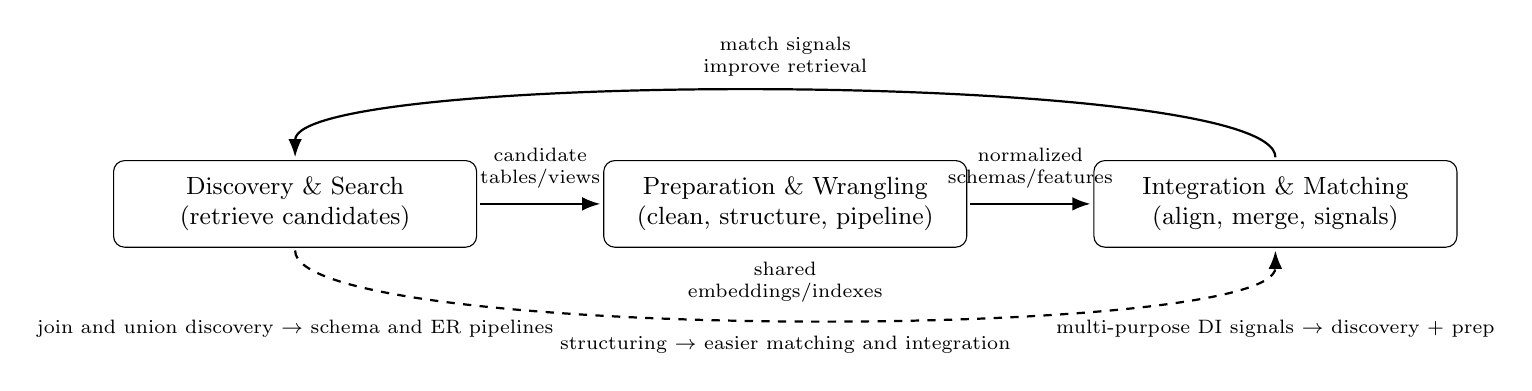
\begin{tikzpicture}[
  font=\small,
  phase/.style={
    draw,
    rounded corners,
    align=center,
    text width=4.4cm,
    minimum height=11mm,
    inner sep=3pt
  },
  arrow/.style={-Latex, thick, shorten <=1pt, shorten >=1pt},
  lbl/.style={font=\scriptsize, align=center}
]

\node[phase] (d) {Discovery \& Search\\(retrieve candidates)};
\node[phase, right=16mm of d] (p) {Preparation \& Wrangling\\(clean, structure, pipeline)};
\node[phase, right=16mm of p] (i) {Integration \& Matching\\(align, merge, signals)};

\draw[arrow] (d) -- node[midway, above=2pt, lbl]{candidate\\tables/views} (p);
\draw[arrow] (p) -- node[midway, above=2pt, lbl]{normalized\\schemas/features} (i);

\coordinate (upR) at ($(i.north)+(0,1.15cm)$);
\coordinate (upL) at ($(d.north)+(0,1.15cm)$);

\draw[arrow]
  (i.north) .. controls (upR) and (upL) .. (d.north)
  node[pos=0.5, above=2pt, lbl]{match signals\\improve retrieval};

\coordinate (dnL) at ($(d.south)+(0,-1.20cm)$);
\coordinate (dnR) at ($(i.south)+(0,-1.20cm)$);

\draw[arrow, dashed]
  (d.south) .. controls (dnL) and (dnR) .. (i.south)
  node[pos=0.5, above=2pt, lbl]{shared\\embeddings/indexes};

\node[below=8mm of d, lbl] {join and union discovery $\rightarrow$ schema and ER pipelines};
\node[below=10mm of p, lbl] {structuring $\rightarrow$ easier matching and integration};
\node[below=8mm of i, lbl] {multi-purpose DI signals $\rightarrow$ discovery + prep};

\end{tikzpicture}
\caption{Cross-phase dependencies. Many systems reuse representations, indexes, or learned signals across discovery, preparation, and integration.}
\label{fig:cross-phase-links}
\end{figure*}

\subsection{Phases Are Connected but Evaluation Is Isolated}
Lake pipelines are coupled. Discovery controls what reaches preparation and matching. Preparation then changes matchability through normalization, structuring, and feature augmentation (adding useful columns). End-to-end methods make this explicit by linking discovery, alignment, and integration in one workflow, or by using shared backbones across discovery tasks \cite{10.1145/3555041.3589732,10.14778/3574245.3574274,10.14778/3659437.3659461,11112882}. Integration outputs (matches, keys, relaxed dependencies) are also reused for retrieval and blocking, creating feedback loops \cite{10184556,10.1145/3588929}. Still, most methods report phase-local metrics only (for example, retrieval precision without final merge quality). This can hide downstream effects. A practical lesson is to report stage-level effectiveness, maintenance cost, and at least one end-to-end outcome together.

Another source of confusion is that methods optimize different objectives, even when they look similar. Discovery may optimize ranking quality. Preparation may optimize consistency or downstream utility. Integration may optimize pair-level accuracy or final-table completeness. Without naming these differences, cross-method comparisons can look cleaner than they are.

\subsection{Ambiguity and User Intent}
In data lakes, ambiguity is structural: weak metadata and heterogeneous representations yield many plausible candidates for one need. Discovery systems address this with interaction and mixed-initiative narrowing, rather than assuming a single correct result \cite{10184768,10.14778/3685800.3685880}. On the integration side, the same data can support multiple valid match interpretations depending on downstream intent \cite{10.1145/3588722}. This challenges the single-ground-truth assumption in many benchmarks. One open problem is intent-conditioned evaluation: vary intent explicitly and report robustness across intents and domains.

\subsection{Scalability, Cost, and Maintenance}
At lake scale, major costs come from \emph{infrastructure}: embedding generation, index construction, and update maintenance. End-to-end stacks and benchmarks show why cost should be reported with effectiveness \cite{10.14778/3685800.3685880,10.14778/3659437.3659448,10.14778/3750601.3750694}. Preparation and integration face similar pressure: pipeline synthesis needs repeated execution and training, and progressive ER uses filtering and scheduling as pay-as-you-go controls \cite{10.1145/3698831,10.1145/3709715,10184692}. Many evaluations still assume static corpora, which hides drift and update behavior. A key direction is incremental maintenance for indexes, embeddings, and tests, with regression checks as lake content evolves.

\subsection{Preparation Needs Safety Checks}
Preparation can improve downstream quality, but gains are not automatic. Repair systems may over-edit or introduce plausible but wrong values, so evaluation should prioritize net error reduction and do-no-harm behavior \cite{10.14778/3675034.3675051}. LM-based curation and structuring make auditability more important because of non-determinism, hallucination risk, and privacy constraints \cite{10.14778/3611540.3611624,10.14778/3574245.3574258}. Structuring methods also show that many lake inputs need multi-step relationalization, not one operator \cite{10.1145/3665252.3665269,10.14778/3626292.3626294,10.14778/3681954.3682019}. In practice, systems need lightweight verification hooks (tests, constraints, sampling checks) that can trigger rollback or human review when confidence is low.

\subsection{Integration Design Choices}
Integration in lakes is not simply ``schema match + join.'' Partial overlaps and nulls require merge semantics that preserve partial facts while maximizing merged evidence. FD-style approaches show that integration operators and semantics shape output quality and can outperform brittle pairwise joins \cite{10.14778/3574245.3574274,10.1145/3555041.3589732}. At the entity level, workflow-first ER shows that filtering, scheduling, and supervision strategies often dominate end-to-end performance and cost \cite{10.1145/3709715,10.1145/3588712,10.1145/3626711,10.1145/3588938}. LM-based matchers help reduce supervision and improve robustness, but they raise calibration, latency, and privacy concerns \cite{10.14778/3742728.3742757}. A key open issue is aligning merge semantics and workflow choices with downstream use, and evaluating those trade-offs directly.

\subsection{Fairness, Privacy, and Governance}
As pipelines become more automated, responsible operation becomes part of system design. Fairness-aware evaluation shows that global accuracy can hide unequal error rates across groups, especially under imbalance and missingness \cite{10.14778/3611479.3611525}. Foundation-model data tasks also raise privacy risks: prompting, serialization, and external APIs can leak sensitive data or violate policy \cite{10.14778/3574245.3574258}. Governance rules also shape what is allowed (joins, attribute exposure, augmentation sources). These rules should be modeled as planning constraints, not added only after the fact. Open problems include fairness auditing beyond the final matcher, privacy-preserving indexing/LLM use, and policy-aware integration planning.

\subsection{Benchmark Gaps and Shared Testbeds}
Shared corpora (shared table collections) and benchmarks improved within-phase comparability, but end-to-end evaluation is still fragmented. GitTables~\cite{10.1145/3588710} and LakeBench~\cite{10.14778/3659437.3659448} standardize parts of discovery, and ER benchmarks support workflow comparison \cite{10184692}. Representation and profiling work also provides reusable signals across tasks \cite{10184556,10.1145/3588929}. Still, few resources jointly cover discovery$\rightarrow$preparation$\rightarrow$integration under updates, changing intent, and explicit cost reporting. A concrete next step is a pipeline testbed that combines workloads, multi-layer ground truth, and audited costs (Table~\ref{tab:benchmark_inventory}).

% ---- Benchmark inventory table ----
\begin{table*}[!htbp]
\centering
\caption{Inventory of shared resources and the gaps they suggest.}
\label{tab:benchmark_inventory}
\tbl
\begin{tabularx}{\textwidth}{@{}p{26mm}p{26mm}Y Y@{}}
\toprule
\textbf{Artifact} & \textbf{Phase(s)} & \textbf{What it enables} & \textbf{Key gaps / limitations} \\
\midrule
GitTables~\cite{10.1145/3588710} &
Discovery (rep.\ learning) &
Large table corpus for training/evaluation of semantic table understanding and retrieval &
Limited evolving-lake settings; not a full end-to-end pipeline workload. \\
\addlinespace[0.25em]
LakeBench~\cite{10.14778/3659437.3659448} &
Discovery (join and union) &
Join/union discovery benchmarks with labeled queries; effectiveness+efficiency comparisons &
Mostly stage-local; limited coupling to preparation/integration outcomes. \\
\addlinespace[0.25em]
Filtering/ER benchmarks~\cite{10184692} &
Integration (ER workflows) &
Systematic evaluation of filtering and scheduling configurations and trade-offs &
Fairness/intent labels are rare; limited policy constraints and multimodal settings. \\
\addlinespace[0.25em]
Reusable signals~\cite{10184556,10.1145/3588929} &
Cross-phase &
Shared representations and profiling signals transferable across tasks &
Need standardized reporting of cost, calibration, and behavior under updates/shift. \\
\bottomrule
\end{tabularx}
\end{table*}

Such a testbed is especially useful in data lakes because failures often occur across stage boundaries, not inside one operator. A discovery method may retrieve semantically relevant but structurally incompatible candidates. A preparation workflow may improve local quality while removing values needed for later matching. An integration workflow may show strong pair-level scores but still produce incomplete or hard-to-use merged outputs. Shared testbeds make these trade-offs easier to observe under one workload.

\subsection{Comparison Clarity Across Phases}
One persistent issue in this literature is that methods often look comparable even when they optimize different targets. Discovery methods usually optimize ranking quality, latency, or index cost. Preparation methods may optimize consistency, error reduction, or downstream model performance. Integration methods may optimize schema-match accuracy, pair-level entity-matching accuracy, or the completeness of the final merged table. These are all reasonable targets, but they are not interchangeable.

Reading these methods together makes the mismatch clear. BLEND and related systems emphasize flexible execution across discovery operators, while CHORUS emphasizes shared semantic signals \cite{11112882,10.14778/3659437.3659461}. Automatic Data Repair shows that results differ depending on whether the goal is consistency or true error reduction \cite{10.14778/3675034.3675051}. DIALITE and ALITE show that integration quality depends not only on local match accuracy, but also on how partial facts are assembled into a final table \cite{10.1145/3555041.3589732,10.14778/3574245.3574274}. So comparisons should always state the optimized target explicitly.

This matters for how survey conclusions are written. It is reasonable to say that recent work improves retrieval quality, lowers supervision cost, or improves merge semantics in a stated setting. It is less safe to claim one line of work is simply better than another without naming the optimization target, output type, and controlled conditions. For this reason, we organize comparisons by output type and phase role, rather than collapsing all methods into one score.

\subsection{Threats to Validity}
Like any survey, this study has limits. Source coverage is one risk: missing methods could bias phase counts and trend claims. To reduce this risk, we searched SIGMOD, PVLDB, and ICDE proceedings and used one inclusion rule across sources. Coding bias is another risk: some methods fit more than one category, so we used one primary-output rule so each method appears once. The 2022--2025 window also narrows the lens, and we state this boundary clearly in Methodology and Related Work. Objective mismatch is another limitation: some works optimize consistency, others optimize retrieval quality or downstream utility, so side-by-side comparison is imperfect. Finally, metric mismatch and limited code/data release make comparisons harder. To avoid overclaiming, we keep phase-specific metrics separate and note where reproducibility is weak.

\subsection{Research Agenda}
The literature suggests five concrete next steps. First, discovery methods should report downstream evidence, not only ranking quality. A practical setup is to fix top-$k$ retrieval and measure integration success on the same workload, then release queries, labels, and retrieved candidate sets. Second, preparation methods should evaluate repair quality and downstream utility together on the same repaired tables, and release dirty--clean pairs, repair outputs, and scripts. Third, integration methods should report pair-level metrics and final-table completeness/consistency on identical inputs, with merged tables and consistency checks. Fourth, update-aware studies are still limited; rerunning workflows on time-sliced snapshots can measure quality drift and maintenance cost together. Fifth, fairness and privacy should be audited across retrieval, preparation, and matching under one protocol, with slice definitions, policy rules, and stage-level audit reports released for reuse.

% ==========================================================
\section{Conclusion}
% ==========================================================
Data lakes lower ingestion barriers for heterogeneous data, but producing \emph{analytics-ready} datasets still requires coordinated discovery, preparation, and integration. In this survey, we organized recent work by output type: ranked candidates for exploration, cleaned and structured data with executable preparation workflows, and alignment outputs or merged datasets. Three broad patterns recur across the literature. Discovery increasingly combines meaning-based representations with practical indexing and interaction. Preparation increasingly produces repeatable workflows, often with language models, but still needs auditability and safety checks. Integration increasingly depends on workflow design, intent awareness, and policy constraints rather than one notion of correctness. A natural next step is pipeline-aware evaluation with shared testbeds that connect stage-level results to end-to-end outcomes under updates, ambiguous intent, and measured cost.


% ==========================================================
\balance
\bibliographystyle{ACM-Reference-Format}
\bibliography{ref}
% ==========================================================

\end{document}
